
Se tienen $k$ vectores ordenados (de menor a mayor), cada uno con $n$ elementos, y queremos
combinarlos en un \'unico vector ordenado (con $kn$ elementos). Una posible alternativa consiste en, utilizando un algoritmo cl\'asico, mezclar los dos primeros vectores, posteriormente mezclar el resultado con el tercero, y as\'i sucesivamente.

\begin{itemize}
    \item ¿Cu\'al ser\'ia el tiempo de ejecuci\'on de este algoritmo?
	\item Diseñe, analice la eficiencia e implemente un algoritmo de mezcla m\'as eficiente, 		  basado en \"divide y vencer\'as\".
	\item Realizar tambi\'en un estudio emp\'irico e h\'ibrido de la eficiencia de ambos 				  algoritmos.
\end{itemize}

\subsection{Estudio preliminar}
Plante\'ando el problema es posible imponer una cota superior te\'orica a la mezcla. Teniendo en cuenta que hay $kn$ elementos, si aplic\'asemos un algoritmo con eficiencia  $O(n)=nlog(n)$ deducimos que podemos encontrar un algoritmo de ordenaci\'on b\'asica con eficiencia $O(k,n)=nklog(nk)$. En este caso estar\'iamos representando los $k$ vectores de $n$ elementos como un \'unico vector, sin aprovechar a\'un el hecho de que parte del \"\ vector\ \" est\'a ordenado.

\subsection{C\'odigo}

\subsubsection{Divide y vencer\'as}

\begin{lstlisting}[language=c++]
// Funcion que llama a todo el algoritmo
int* MezclaDyV(int** vectors, int n_vec, int n_elem){
  int * full_vector = GeneraVector(vectors, n_vec, n_elem); // Generamos el vector a devolver
  MergeKPartitions(full_vector, n_elem, 0, n_vec*n_elem-1); // Aplicamos la particion y mezcla

  return full_vector;
}
\end{lstlisting}

\begin{lstlisting}[language=c++]
// Funcion que genera un vector a partir de una matriz, colocando cada vector
// seguido de otro.
int * GeneraVector(int** &matriz, int n_vec, int n_elem){
  int* vector = new int[n_vec*n_elem];

  for (int i=0; i<n_vec; ++i){
    for (int j=0; j<n_elem; ++j){
      vector[i*n_elem+j] = matriz[i][j];
    }
  }

  return vector;
}
\end{lstlisting}

\begin{lstlisting}[language=c++]
// Funcion que hace la particion del vector, teniendo en cuenta donde empieza,
// donde termina y el numero de elementos de la particion, y devuelve ese trozo
// ya ordenado
void MergeKPartitions(int* &vector, int n_elem, int ini, int fin){
  int size = fin - ini + 1;
  int partitions = size/n_elem;
  // Caso base: Si hay 2 particiones de igual tamanio, las mezcla
  if(partitions == 2){
    Merge(vector, ini, ini+n_elem, fin);
  }
  // Si hay mas de dos particiones:
  else if(partitions > 2){
    int division = ini + (partitions/2)*n_elem; // Calculo de la division
    // Aqui es basicamente donde aplicamos divide y venceras, el cual nos acaba
    // proporcionando la eficiencia deseada para esta situacion.
    MergeKPartitions(vector, n_elem, ini, division-1);  // Llamada al primer conjunto de particiones
    MergeKPartitions(vector, n_elem, division, fin);    // Llamada al segundo conjunto de particiones
    Merge(vector, ini, division, fin);  // Mezclamos los dos conjuntos de particiones, ya ordenados
  }
}
\end{lstlisting}

\begin{lstlisting}[language=c++]
// Funcion que mezcla dos vectores ordenados en uno ordenado
void Merge(int* &vector, int ini, int pivot, int fin){
  int size = fin-ini+1;
  int f_count = 0, s_count = 0;// Contadores de cada vector
  int selected;
  int* aux = new int[size];

  // Hasta que agotemos el tamanio del vector auxiliar
  for (int i=0; i<size; ++i){
    // Si hemos agotado el primer vector:
    if(ini+f_count == pivot){
      selected = vector[pivot+s_count];
      s_count++;
    }
    // Si hemos agotado el segundo:
    else if(s_count+pivot == fin+1){
      selected = vector[ini+f_count];
      f_count++;
    }
    // En cualquier otro caso:
    else{
      // Si el del primer vector es mayor que el del segundo:
      if(vector[ini+f_count] <= vector[pivot+s_count]){
        selected = vector[ini+f_count];
        f_count++;
      }
      // Si es al reves:
      else{
        selected = vector[pivot+s_count];
        s_count++;
      }
    }
    // Asignamos valor a la posicion correspondiente del vector
    aux[i] = selected;
  }
  // Asignamos el vector auxiliar al trozo del vector real
  for (int i=0; i<size; ++i){
    vector[ini+i] = aux[i];
  }
  delete[] aux;
}
\end{lstlisting}

\subsubsection{Fuerza bruta}

\begin{lstlisting}[language=c++]
int* MezclaNoDyV(int** M, int num_vec, int num_elem){
  int* vec_indices = new int[num_vec]; //Vector que almacena los indices
  for (int i=0; i<num_vec; ++i)
    vec_indices[i]=0;

  int pos_escritas = 0; //Numero de posiciones escritas
  const int MAX_POS_ESCRITAS = num_vec*num_elem; //Tope de las posiciones que se pueden escribir (n*k)
  int* vec_ordenado = new int[MAX_POS_ESCRITAS]; //Variable donde se va almacenando el vector resultante ordenado.

  while (pos_escritas < MAX_POS_ESCRITAS){
    int pos_min = f_pos_min(vec_indices, M, num_vec);
    vec_ordenado[pos_escritas] = M[pos_min][vec_indices[pos_min]];
    if (vec_indices[pos_min] >= num_elem-1)
      vec_indices[pos_min] = -1;
    else
      ++vec_indices[pos_min];
    ++pos_escritas;
  }

  delete[] vec_indices;
  return vec_ordenado;
}
\end{lstlisting}

\begin{lstlisting}[language=c++]

//Funcion que calcula el minimo de entre los elementos apuntados por los indices

int f_pos_min(int* vec_indices, int** M, int num_vec){
  int pos_min = 0;
  while((vec_indices[pos_min] <0) && (pos_min < num_vec))
    ++pos_min;
  for (int i=pos_min+1; i<num_vec; ++i){
    if (vec_indices[i] >= 0){
      if (M[i][vec_indices[i]] < M[pos_min][vec_indices[pos_min]])
        pos_min = i;
    }
  }
  return pos_min;
}
\end{lstlisting}

\subsection{Tiempo de ejecuci\'on}


\subsection{Estudio emp\'irico e h\'ibrido}

\subsubsection{Mezcla con furza bruta}
\begin{figure}[htb] 
\centering
	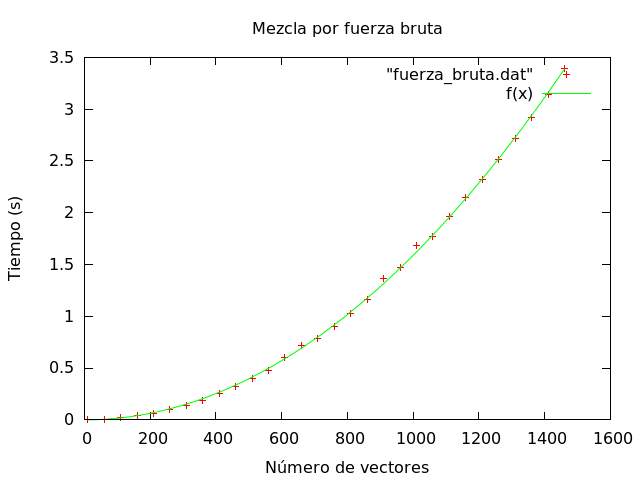
\includegraphics[width=0.6\textwidth]{../Obligatorio/Graficas/fuerza_bruta_kvectores.png}
	\caption{Fuerza bruta con 100 elementos cada vector} 
	\label{fig:f_kvectores} 
\end{figure}

\begin{figure}[htb] 
\centering
	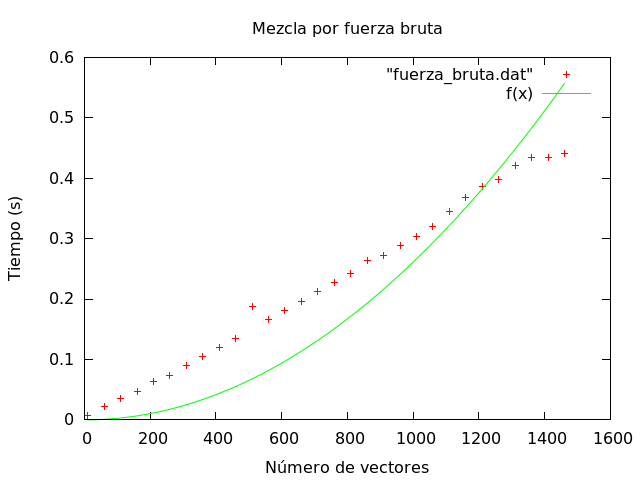
\includegraphics[width=0.6\textwidth]{../Obligatorio/Graficas/fuerza_bruta_nelementos.png}
	\caption{Fuerza bruta con 100 vectores} 
	\label{fig:f_nelementos} 
\end{figure}
\newpage


\subsubsection{Mezcla con divide y vencer\'as}
\begin{figure}[htb] 
\centering
	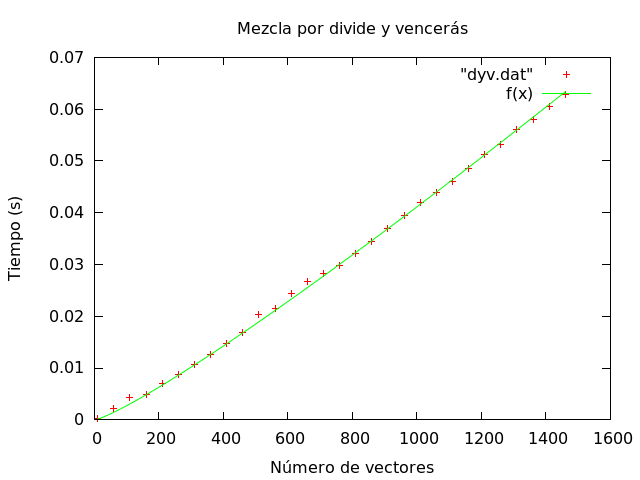
\includegraphics[width=0.6\textwidth]{../Obligatorio/Graficas/dyv_kvectores.png}
	\caption{Divide y vencerás con 100 elementos cada vector} 
	\label{fig:d_kvectores} 
\end{figure}

\begin{figure}[htb] 
\centering
	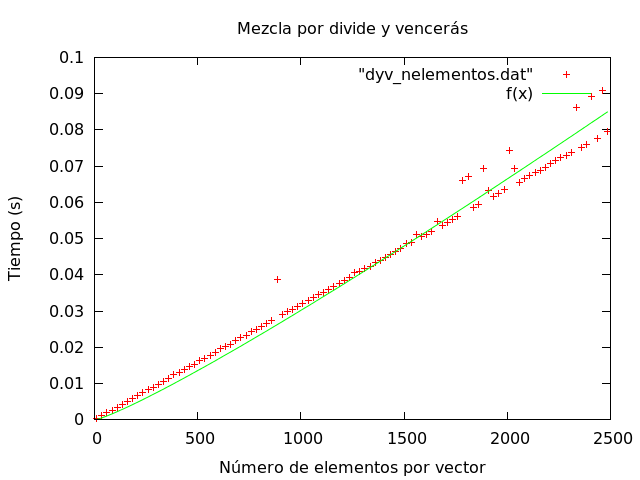
\includegraphics[width=0.6\textwidth]{../Obligatorio/Graficas/dyv_nelementos.png}
	\caption{Divide y vencerás con 100 vectores} 
	\label{fig:d_nelementos} 
\end{figure}
\newpage

\subsubsection{Comparativa}
\begin{figure}[htb] 
\centering
	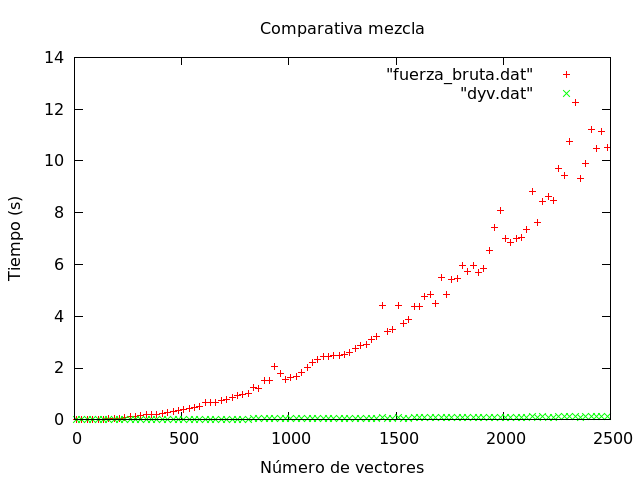
\includegraphics[width=0.6\textwidth]{../Obligatorio/Graficas/comparativa_kvectores.png}
	\caption{Comparativa con 100 elementos cada vector} 
	\label{fig:comp_kvectores} 
\end{figure}

\begin{figure}[htb] 
\centering
	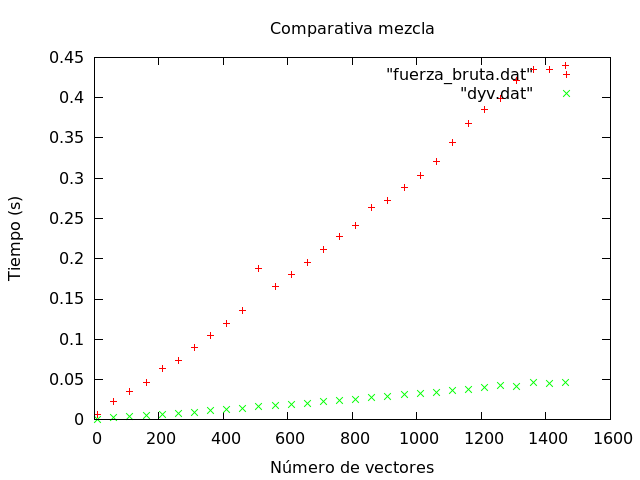
\includegraphics[width=0.6\textwidth]{../Obligatorio/Graficas/comparativa_nelementos.png}
	\caption{Comparativa con 100 vectores} 
	\label{fig:comp_nelementos} 
\end{figure}
\newpage



